\documentclass[
    table,
    12pt,
    oneside,
    a4paper,
    italian
]{book}

\PassOptionsToPackage{dvipsnames}{xcolor} % colori PDF/A

\usepackage{colorprofiles}
% PDF/A
% validate in https://www.pdf-online.com/osa/validate.aspx
\usepackage[a-1a,mathxmp]{pdfx}[2018/12/22]
\usepackage[T1]{fontenc}
\usepackage[utf8]{inputenc}
\usepackage[italian]{babel}
\usepackage{bookmark}
\usepackage{caption}
\usepackage{comment}
\usepackage{chngpage, calc} % centra il frontespizio
\usepackage{emptypage} % pagine vuote senza testatina e piede di pagina
\usepackage{epigraph} % per epigrafi
\usepackage{indentfirst} % rientra il primo paragrafo di ogni sezione
\usepackage{graphicx} % immagini
\usepackage[pdfa]{hyperref} % collegamenti ipertestuali
\usepackage{mparhack,relsize}  % finezze tipografiche
\usepackage{nameref} % visualizza nome dei riferimenti
\usepackage[font=small]{quoting} % citazioni
\usepackage{subfig} % sottofigure, sottotabelle
\usepackage[italian]{varioref} % riferimenti completi della pagina
\usepackage{longtable} % tabelle su più pagine
\usepackage[toc, acronym, automake]{glossaries}
\usepackage[backend=biber, style=verbose-ibid, hyperref, backref]{biblatex}
\usepackage{lmodern}
\usepackage[top=2.75cm, bottom=2.75cm, right=3cm, left=3.75cm]{geometry} % 1in+17pt+0.6cm
\usepackage{fancyhdr}
\usepackage{lipsum}
\usepackage{graphicx}
\usepackage{float}
\usepackage{setspace}
\usepackage{titlesec}
\usepackage{minted} % https://it.overleaf.com/learn/latex/Code_Highlighting_with_minted
\usepackage{xcolor}
\usepackage{csquotes} % gestisce automaticamente i caratteri (")
\usepackage{etoolbox}
\usepackage[table,xcdraw]{xcolor}
\usepackage{changepage}
% Load variables
\newcommand{\myUni}{Università degli Studi di Padova}
\newcommand{\myDepartment}{Dipartimento di Matematica ``Tullio Levi-Civita''}
\newcommand{\myFaculty}{Corso di Laurea in Informatica}
\newcommand{\myTitle}{Una libreria per la visualizzazione di dashboard dinamiche.​}
\newcommand{\myDegree}{Tesi di Laurea Triennale}
\newcommand{\profTitle}{Prof.}
\newcommand{\myProf}{Baldan Paolo}
\newcommand{\graduateTitle}{Laureando}
\newcommand{\myName}{Bresolin Gianluca}
\newcommand{\myStudentID}{2034316}
\newcommand{\myAA}{2023-2024}
\newcommand{\myLocation}{Padova}
\newcommand{\myTime}{Luglio 2024}
% Acronyms

% Glossary

\newglossaryentrywithacronym{SDK}{SDK}{Software Development Kit}{
    Un \textit{Software Development Kit (SDK)} è un insieme di strumenti di sviluppo software riuniti in un unico pacchetto installabile.
    Gli SDK sono progettati per semplificare il processo di sviluppo di applicazioni, fornendo librerie, strumenti di sviluppo, documentazione e esempi di codice
}

\newglossaryentrywithacronym{FCP}{FCP}{First Contentful Paint}{
    Il \textit{First Contentful Paint (FCP)} è una metrica che misura il tempo dal momento in cui una pagina inizia il caricamento fino al momento in cui qualsiasi parte
    del contenuto della pagina viene resa visibile sullo schermo
}

\newglossaryentrywithacronym{SVG}{SVG}{Scalable Vector Graphics}{
    L'\textit{SVG (Scalable Vector Graphics)} è un formato di file basato su \textit{XML} per descrivere immagini vettoriali bidimensionali.
    Questo formato permette la rappresentazione di grafica vettoriale con alta precisione, consentendo lo zoom e il ridimensionamento senza perdita di qualità.
    Gli SVG sono utilizzati ampiamente nel \textit{web design} e nelle applicazioni grafiche grazie alla loro scalabilità e al supporto per interattività e animazioni tramite script e fogli di stile
}

\newglossaryentrywithacronym{API}{API}{Application Programming Interface}{
    Un'\textit{API (Application Programming Interface)} è un insieme di definizioni e protocolli che permettono a diversi software di comunicare tra loro.
    Le API forniscono un'interfaccia standardizzata che consente agli sviluppatori di accedere a funzionalità e servizi di un altro software, sistema operativo, libreria o
    framework senza conoscere i dettagli della loro implementazione
}

\newglossaryentrywithacronym{TTI}{TTI}{Time to Interactive}{
    Il \textit{Time to Interactive (TTI)} è una metrica che misura il tempo necessario affinché una pagina web diventi completamente interattiva, cioè quando è possibile
    interagire con tutti gli elementi principali della pagina senza ritardi significativi
}

\newglossaryentry{open-source}{
    name={Open-Source},
    text={open-source},
    sort=open-source,
    description={Il termine \textit{open-source} si riferisce a un tipo di software il cui codice sorgente è disponibile per l'uso, la modifica e la distribuzione da parte di chiunque.
            Questo modello promuove la collaborazione e la trasparenza nello sviluppo software}
}

\newglossaryentry{refactoring}{
    name={Refactoring},
    text={refactoring},
    sort=refactoring,
    description={Il refactoring è il processo di ristrutturazione del codice sorgente di un programma senza modificarne il comportamento esterno.
            L'obiettivo è migliorare la leggibilità, la manutenibilità e la riduzione della complessità del codice}
}

\newglossaryentry{package}{
    name={Package},
    text={package},
    sort=package,
    description={Un \textit{package} è un insieme di moduli o classi che vengono raggruppati insieme e distribuiti come una singola unità.
            I pacchetti facilitano la gestione e la distribuzione del software, includendo tutte le dipendenze necessarie}
}

\newglossaryentry{bundle}{
    name={Bundle},
    text={bundle},
    sort=bundle,
    description={Un \textit{bundle} è un pacchetto che contiene diversi file e risorse che vengono aggregati insieme per essere distribuiti come un'unica unità.
            In ambito web, un \textit{bundle} può includere file \textit{JavaScript}, \textit{CSS} e immagini}
}

\newglossaryentry{backend}{
    name={Backend},
    text={backend},
    sort=backend,
    description={Il \textit{backend} si riferisce alla parte server di un'applicazione, che gestisce la logica, le operazioni di database, l'autenticazione degli utenti e
            altre funzionalità che non sono visibili direttamente dall'utente finale}
}

\newglossaryentry{responsive}{
    name={Responsive},
    text={responsive},
    sort=responsive,
    description={Il termine \textit{responsive} si riferisce a un design che è in grado di adattarsi a diverse dimensioni dello schermo e dispositivi,
            offrendo un'esperienza utente ottimale, indipendentemente dal dispositivo utilizzato}
}

\newglossaryentry{rendering}{
    name={Rendering},
    text={rendering},
    sort=rendering,
    description={Il rendering è il processo di generazione di un'immagine o di una visualizzazione a partire da un modello o da un insieme di dati.
            In ambito web, il rendering si riferisce alla trasformazione del codice \textit{HTML, CSS} e \textit{JavaScript} in una pagina web visibile e interattiva.
            Il rendering può essere eseguito lato \textit{client}, nel \textit{browser},
            o lato \textit{server}, prima che la pagina venga inviata al \textit{client}}
}

\newglossaryentry{runtime}{
    name={Runtime},
    text={runtime},
    sort=runtime,
    description={Il \textit{runtime} si riferisce al periodo di tempo durante il quale un programma è in esecuzione. Il termine viene anche utilizzato per indicare un ambiente o
            una libreria che supporta l'esecuzione di un programma, fornendo servizi come la gestione della memoria e l'esecuzione del codice}
}

\newglossaryentry{super-set}{
    name={Super-Set},
    text={super-set},
    sort=super-set,
    description={Un super-set è un insieme che contiene tutti gli elementi di un altro insieme, detto sottoinsieme. Nel contesto della programmazione, un linguaggio o un \textit{framework}
            può essere considerato un \textit{super-set} se include tutte le funzionalità di un altro linguaggio o \textit{framework}, aggiungendo ulteriori caratteristiche e capacità.}
}

\newglossaryentry{peerdependency}{
    name={Peer Dependency},
    text={peer-dependency},
    sort=peerdependency,
    description={Una \textit{peer dependency} è una dipendenza di un modulo che non viene installata automaticamente, ma che deve essere fornita dall'ambiente in cui il modulo stesso è eseguito.
            Questo tipo di dipendenza è utilizzato per garantire che i moduli condividano una singola istanza di una libreria comune, evitando problemi di incompatibilità e ridondanza.}
}

\newglossaryentry{bundler}{
    name={Bundler},
    text={bundler},
    sort=bundler,
    description={Un \textit{bundler} è uno strumento utilizzato nello sviluppo web per combinare diversi file e risorse, come \textit{JavaScript}, \textit{CSS} e immagini, in un unico
            file o in un insieme di file più ridotto. Questo processo migliora l'efficienza del caricamento delle pagine web riducendo il numero di richieste HTTP necessarie}
}

\newglossaryentry{tree-shaking}{
    name={Tree-Shaking},
    text={tree-shaking},
    sort=tree-shaking,
    description={Il \textit{tree-shaking} è una tecnica di ottimizzazione del codice utilizzata dai \textit{bundler} per rimuovere codice inutilizzato dai file JavaScript. Questo processo
            analizza le dipendenze del codice per identificare e eliminare le parti che non sono effettivamente utilizzate, riducendo la dimensione finale del \textit{bundle} e migliorando le
            prestazioni delle applicazioni web}
}

\newglossaryentry{memoizzato}{
    name={Memoizzato},
    text={memoizzato},
    sort=memoizzato,
    description={Il termine \textit{memoizzato} si riferisce a una tecnica di ottimizzazione che memorizza il risultato di una funzione o di un calcolo in modo da poterlo riutilizzare
            in seguito senza doverlo ricalcolare. Questo approccio migliora le prestazioni dell'applicazione riducendo il tempo di esecuzione e l'utilizzo delle risorse}
}

\newglossaryentry{frontend}{
    name={Frontend},
    text={frontend},
    sort=frontend,
    description={Il \textit{frontend} si riferisce alla parte visibile di un'applicazione, che interagisce direttamente con l'utente finale. Questa parte dell'applicazione gestisce l'interfaccia
            utente, la presentazione dei dati e le interazioni con l'utente}
}

\newglossaryentry{repository}{
    name={Repository},
    text={repository},
    sort=repository,
    description={Un \textit{repository} è un archivio centralizzato e strutturato per la conservazione, la gestione e il controllo di versioni di codice sorgente, documentazione e altri file correlati
            a un progetto software. I repository possono essere ospitati su server locali o remoti e sono spesso gestiti tramite sistemi di controllo versione, consentendo agli sviluppatori di collaborare,
            tracciare modifiche, gestire diramazioni (\textit{branch}) e fusioni (\textit{merge}), mantenendo una cronologia accurata dello sviluppo del software}
}

\newglossaryentry{framework}{
    name={Framework},
    text={framework},
    sort=framework,
    description={Un \textit{framework} è un insieme di librerie, strumenti e linee guida che forniscono una struttura e un'infrastruttura per lo sviluppo di applicazioni software.
            I \textit{framework} semplificano il processo di sviluppo fornendo funzionalità comuni, standardizzando le pratiche di programmazione e riducendo la complessità del codice}
}

\newglossaryentry{memory leak}{
    name={Memory Leak},
    text={memory leak},
    sort=memoryleak,
    description={Un \textit{memory leak} (perdita di memoria) è una condizione anomala in cui un programma software, durante la sua esecuzione, non rilascia correttamente la memoria che ha allocato.
            Questo comportamento porta ad un utilizzo inefficiente della memoria disponibile, riducendone progressivamente la quantità fino a potenzialmente esaurire tutte le risorse di memoria del sistema.
            I \textit{memory leak} sono spesso causati da errori di programmazione, come la mancata deallocazione di memoria dinamica o riferimenti pendenti a oggetti non più utilizzati}
}

\newglossaryentry{mock}{
    name={Mock},
    text={mock},
    sort=mock,
    description={Un \textit{mock} è un oggetto simulato o fittizio che viene utilizzato al posto di un oggetto o una funzione reale durante i test software. I \textit{mock} vengono utilizzati per simulare il comportamento
            di un oggetto o funzione reale, consentendo ai test di verificare il funzionamento del codice in modo controllato e prevedibile, limitando le responsabilità testate alle sole logiche specifiche}
}

\newglossaryentry{munging}{
    name={Munging},
    text={munging},
    sort=munging,
    description={Il \textit{munging} è una tecnica di trasformazione dei dati che modifica o oscura i dati in modo da renderli irriconoscibili o incomprensibili per chi non è autorizzato a visualizzarli.
            Il \textit{munging} viene spesso utilizzato per proteggere i dati sensibili o per nascondere informazioni personali, come indirizzi email o numeri di telefono, sostituendo i caratteri con simboli o codici.
            Questa tecnica viene inoltre utilizzata per ottimizzare il codice sorgente, riducendo la dimensione dei file}
}

% Define custom colors
\definecolor{hyperColor}{HTML}{0B3EE3}
\definecolor{tableGray}{HTML}{F5F5F7}

% Set line height
\linespread{1.2}

% Custom hyphenation rules
\hyphenation {
    e-sem-pio
    ex-am-ple
}

% Images path
\graphicspath{{img/}}

% Force page color, as some editors set a grayish color as default
\pagecolor{white}

% Better spacing for footnotes
\setlength{\skip\footins}{5mm}
\setlength{\footnotesep}{5mm}

\setlength{\headheight}{14.5pt}
\addtolength{\topmargin}{-2.45pt}

% Add a subscript G to a glossary entry
\newcommand{\glox}{\textsubscript{\textbf{\textit{G }}}}

% If the subscript G is followed by a punctuation character, or anything else, you need to use \gloxspacing to prevent rendering issues, where the characters collide. Example in Chapter 7
\newcommand{\gloxspacing}{\hspace{-0.3em}}

% Improvements the paragraph command
\titleformat{\paragraph}
{\normalfont\normalsize\bfseries}{\theparagraph}{1em}{}
\titlespacing*{\paragraph}
{0pt}{3.25ex plus 1ex minus .2ex}{1.5ex plus .2ex}

% Define use case environment
\newcounter{usecasecounter} % define a counter
\setcounter{usecasecounter}{0} % set the counter to some initial value
% Parameters
% #1: ID
% #2: Nome
\newenvironment{usecase}[2]{
    \renewcommand{\theusecasecounter}{\usecasename #1}  % this is where the display of the counter is overwritten/modified
    \refstepcounter{usecasecounter} % increment counter
    \vspace{2em}
    \par \noindent % start new paragraph
    {\normalsize \textbf{\usecasename #1: #2}} % display the title before the content of the environment is displayed
    \vspace{.5em}
}{
    \medskip
}
\newcommand{\usecasename}{UC}
\newcommand{\usecaseactors}[1]{\textbf{\\Attori Principali:} #1}
\newcommand{\usecasepre}[1]{\textbf{\\Precondizioni:} #1}
\newcommand{\usecasedesc}[1]{\textbf{\\Descrizione:} #1}
\newcommand{\usecasepost}[1]{\textbf{\\Postcondizioni:} #1}
\newcommand{\usecasealt}[1]{\textbf{\\Scenario Alternativo:} #1}

% Define risks environment
\newcounter{riskcounter} % define a counter
\setcounter{riskcounter}{0} % set the counter to some initial value
% Parameters
% #1: Title
\newenvironment{risk}[1]{
    \refstepcounter{riskcounter} % increment counter
    \par \noindent % start new paragraph
    \textbf{\arabic{riskcounter}. #1} % display the title before the content of the environment is displayed
}{
    \par\medskip
}
\newcommand{\riskname}{Rischio}
\newcommand{\riskdescription}[1]{\textbf{\\Descrizione:} #1.}
\newcommand{\risksolution}[1]{\textbf{\\Soluzione:} #1.}

% Apply fancy styling to pages
\pagestyle{fancy}
\fancyhf{}
\fancyhead[L]{\leftmark} % Places Chapter N. Chatper title on the top left
\fancyfoot[C]{\thepage} % Page number in the center of the footer

% Adds a blank page while increasing the page number
\newcommand\blankpage{
    \clearpage
    \begingroup
    \null
    \thispagestyle{empty}
    \hypersetup{pageanchor=false}
    \clearpage
    \endgroup
}

% Increase page numbering
\newcommand\increasepagenumbering{
    \addtocounter{page}{+1}
}

% Make glossaries and bibliography
\makeglossaries
\bibliography{references/bibliography}
\defbibheading{bibliography} {
    \cleardoublepage
    \phantomsection
    \addcontentsline{toc}{chapter}{\bibname}
    \chapter*{\bibname\markboth{\bibname}{\bibname}}
}

% Code blocks handling w/ table of codes
\makeatletter
\ifdefined\NR@chapter
    \expandafter\@firstoftwo
\else
    \expandafter\@secondoftwo
\fi{\patchcmd\NR@chapter}{\patchcmd\@chapter}
{\addtocontents{lot}{\protect\addvspace{10\p@}}}
{\addtocontents{lot}{\protect\addvspace{10\p@}}%
\addtocontents{lol}{\protect\addvspace{10\p@}}}
{}{}
\makeatother

\renewcommand\listingscaption{Codice}
\renewcommand\listoflistingscaption{Elenco dei codici sorgenti}
\counterwithin*{listing}{chapter}
\renewcommand\thelisting{\thechapter.\arabic{listing}}

% Set up hyperlinks
\hypersetup{
    colorlinks=true,
    linktocpage=true,
    pdfstartpage=1,
    pdfstartview=,
    breaklinks=true,
    pdfpagemode=UseNone,
    pageanchor=true,
    pdfpagemode=UseOutlines,
    plainpages=false,
    bookmarksnumbered,
    bookmarksopen=true,
    bookmarksopenlevel=1,
    hypertexnames=true,
    pdfhighlight=/O,
    allcolors = hyperColor
}

% Set up captions
\captionsetup{
    tableposition=top,
    figureposition=bottom,
    font=small,
    format=hang,
    labelfont=bf
}

\date{}

\hypersetup{pdfstartview=}
\begin{document}
    \frontmatter
    \begin{titlepage}
    \begin{center}
        \begin{Large}
            \textbf{\myUni}\\
        \end{Large}

        \vspace{5pt}

        \begin{large}
            \textsc{\myDepartment}\\
        \end{large}

        \vspace{5pt}

        \begin{large}
            \textsc{\myFaculty}\\
        \end{large}

        \vspace{25pt}
        
        \begin{figure}[htbp]
            \centering
            
\includegraphics[alt={Emblema dell'Università degli Studi di Padova}, height=6cm]{img/logo_unipd.jpeg}
        \end{figure}

        
        \begin{Large}
            \textbf{\myTitle}\\
        \end{Large}

        \vspace{5pt}

        \begin{large}
            \textit{\myDegree}\\
        \end{large}

        \vspace{50pt}
        
        \begin{normalsize}
            \begin{flushleft}
                \textit{Relatore}\\
                \profTitle\ \myProf
            \end{flushleft}

            \vspace{-48pt}
            
            \begin{flushright}
                \textit{\graduateTitle}\\
                \myName\\
                Matricola \myStudentID
            \end{flushright}
        \end{normalsize}

        \vspace*{\fill}
        
        \line(1, 0){338} \\
        \begin{normalsize}
            \textsc{Anno Accademico \myAA}
        \end{normalsize}
    \end{center}
\end{titlepage}

    \increasepagenumbering % increase the page numbrering by 1, in order to cout the frontispiece
    \clearpage
\phantomsection
\thispagestyle{empty}
\hfill
\vfill

{\small\noindent\textcopyright\ \myName, \myTime. Tutti i diritti riservati. \myDegree: ``\textit{\myTitle}'', \myUni, \myDepartment.}
    \cleardoublepage
\phantomsection
\pdfbookmark{Ringraziamenti}{Ringraziamenti}

\begin{flushright}{
        \slshape
        ``''} \\
    \medskip
    --- .
\end{flushright}

\begingroup
\let\clearpage\relax
\let\cleardoublepage\relax
\let\cleardoublepage\relax

\chapter*{Ringraziamenti}

\noindent Desidero esprimere la mia gratitudine al professor \myProf, mio relatore, per l'aiuto e il sostegno che mi ha dato durante la stesura dell'elaborato.

\vspace{0.35cm}

\noindent Vorrei anche ringraziare, con affetto, i miei genitori per il loro sostegno, il grande aiuto e la loro presenza in ogni momento durante gli anni di studio.

\vspace{0.35cm}

\noindent Desidero poi ringraziare i miei amici per i bellissimi anni trascorsi insieme e le mille avventure vissute.

\vspace{0.75cm}

\noindent{\myLocation, \myTime}
\hfill \textit{\myName}

\endgroup

    \cleardoublepage
\phantomsection
\pdfbookmark{Compendio}{Compendio}
\begingroup
\let\clearpage\relax
\let\cleardoublepage\relax
\chapter*{Sommario}

Il presente documento descrive il lavoro svolto durante il periodo di stage, \lipsum[1]

\endgroup
\vfill

    \cleardoublepage
\pdfbookmark{\contentsname}{tableofcontents}
\setcounter{secnumdepth}{5}
\setcounter{tocdepth}{5}     

\tableofcontents
\clearpage

\begingroup
    \let\clearpage\relax
    \let\cleardoublepage\relax
    \let\cleardoublepage\relax

    % Figures list
    \phantomsection
    \pdfbookmark{\listfigurename}{lof}
    \listoffigures
    \vspace*{8ex}

    % Tables list
    \phantomsection
    \pdfbookmark{\listtablename}{lot}
    \listoftables
\endgroup

\begingroup
    % Code list
    \phantomsection
    \pdfbookmark{\listoflistingscaption}{lol}
    \listoflistings
\endgroup

\cleardoublepage
    \printglossary[type=\acronymtype, title=Acronimi e abbreviazioni, toctitle=Acronimi e abbreviazioni]
    \printglossary[type=main, title=Glossario, toctitle=Glossario]
    \blankpage % example of a blank page that also increases the page couter by 1

    \mainmatter
    \chapter{Introduzione}
\label{chap:introduzione}

% * INTRODUZIONE

% - Breve descrizione del progetto
% - Principali problematiche
% - Soluzione scelta
% - Strumenti utilizzati
% - Descrizione del prodotto ottenuto
% - Struttura del resto della relazione

\section{L'azienda}
Lo stage è stato svolto presso l'azienda Datasoil S.r.l. situata nei dintorni della stazione ferroviaria di Padova.
Fondata nel XXXX, Datasoil S.r.l. è un'azienda di prodotto che si dedica allo sviluppo di piattaforme per l'industria 4.0,
smart building e smart city.
L'obiettivo dell'azienda è integrare informazioni ed eventi provenienti dai vari livelli aziendali per creare insight proattivi
in tempo reale, garantendo che le informazioni corrette raggiungano le persone giuste al momento più opportuno.
Il punto di partenza è la spazialità aziendale e tutti gli asset che risiedono all'interno di essa, da cui
provengono tutti i dati che vengono analizzati trasversalmente grazie a sempre più persone e dispositivi connessi.
Da qui il nome dell'azienda, Datasoil: fare le informazioni da questo suolo fertile di dati da cui siamo circondati.

\begin{figure}[H]
      \centering
      
\includegraphics[alt={Logo Datasoil S.r.l.}, width=0.25\columnwidth]{img/datasoil_logo.jpg}
      \caption{Logo Datasoil S.r.l.}
      \label{fig:datasoil}
\end{figure}

\section{L'idea}
\subsection{Il contesto applicativo}
L'azienda Datasoil S.r.l., essendo un'azienda di prodotto, nasce con l'idea di proporre servizi di monitoraggio e controllo
di impianti industriali, smart building e smart city, offrendo come principale prodotto la piattaforma SYN.

\begin{figure}[H]
      \centering
      
\includegraphics[alt={Logo SYN}, width=0.25\columnwidth]{img/syn_logo.jpg}
      \caption{Logo SYN}
      \label{fig:syn}
\end{figure}

SYN è una piattaforma di monitoraggio e controllo di impianti industriali che raccoglie dati da sensori e dispositivi
distribuiti all'interno di un impianto o su più stabilimenti, permettendo di visualizzare in tempo reale lo stato di
funzionamento dei vari asset, di analizzare i dati raccolti e di attuare azioni di controllo o segnalazione tramite
ticketing. All'interno della piattaforma, a seconda dei piani attivati dal cliente, è possibile visualizzare dashboard dinamiche
in merito ad informazioni filtrate e aggiornate live, permettendo di raggiungere una panoramica completa dello stato dei vari
asset monitorati in modo rapido, intuitivo ed efficace, grazie all'utilizzo di molteplici grafici e widget.

\subsection{Il progetto}
Il progetto svolto durante lo stage consiste nello sviluppo di una libreria TypeScript di componenti per la creazione di dashboard dinamiche.
Questo è stato realizzato tramite il refactoring e l'ottimizzazione di un tool grafico preesistente, integrato nei vari prodotti di Datasoil S.r.l.,
tra cui \textit{SYN}. La libreria è stata implementata a partire da una libreria open-source utilizzata in \textit{Redash},
una piattaforma per la creazione di dashboard dinamiche tramite interrogazioni sulle fonti di dati configurate all'interno del servizio. \newline
L'esigenza di tale progetto nasce dalla necessità da parte di Datasoil S.r.l. di avere una libreria grafica aggiornata alle versioni
correnti delle dipendenze utilizzate, raggiungendo una maggior performance e una maggiore manutenibilità del codice rispetto alla versione
preesistente, riducendo dove possibile le dipendenze esterne e introducendo migliorie grafiche e funzionali.

\section{Principali problematiche}
Durante l'analisi iniziale della libreria preesistente in uso all'interno dei prodotti di Datasoil S.r.l., sono emerse a fronte di una
revisione del codice sorgente alcune problematiche legate alla manutenibilità e alla performance del tool grafico.

\subsection{Dipendenze obsolete}
La libreria preesistente utilizzava versioni obsolete delle dipendenze esterne, con conseguente rallentamento delle prestazioni in termini
di utilizzo di spazio e di tempo di caricamente delle risorse, data l'assenza di ottimizzazioni e di aggiornamenti del codice sorgente. \newline
Essendo inoltre la libreria preesistente basata su una versione della piattaforma \textit{Redash}, i moduli utilizzati il più delle volte
rappresentavono alternative a quelli già utilizzati all'interno dei prodotti Datasoil S.r.l., creando una dipendenze non necessarie che
causavano un aumento delle dimensioni del SDK utilizzato per la creazione delle dashboard.

\subsection{Manutenibilità del codice}
Il codice sorgente della libreria preesistente, essendo stato sviluppato a fronte di una esigenza specifica dell'azienda Datasoil S.r.l.,
risultava essere poco manutenibile e assente di documentazione. \newline
Inoltre, la libreria utilizzata da \textit{Redash}, inizialmente era stata sviluppata in JavaScript, subendo solo successivamente un
refactoring in TypeScript: questo refactoring non è però avvenuto con l'introduzione di interfacce e tipi, bensì con la semplice aggiunta
di tipi \textit{any} per le variabili e i parametri delle funzioni, rendendo il codice poco leggibile e difficile da mantenere.

\subsection{Componenti inutilizzate}
In quanto la libreria preesistente fosse realizzata a partire dal modulo utilizzato dalla piattaforma \textit{Redash}, non tutti i componenti presenti
in essa trovavano utilizzo all'interno dei prodotti realizzati da Datasoil S.r.l.: questo in gran parte era dovuto da una offerta di grafici inopportuni
per quello che è il contesto applicativo dell'azienda.

\subsection{Assenza di funzionalità}
La libreria preesistente non soddisfaceva pienamente le esigenze dei clienti di Datasoil S.r.l., mancando di alcune funzionalità fondamentali.
Questa limitazione ha reso necessario un intervento di refactoring per colmare le lacune e migliorare le prestazioni complessive.

\section{Soluzione scelte}
Per risolvere le problematiche emerse durante l'analisi iniziale della libreria preesistente, si è optato per il refactoring e l'ottimizzazione
del codice sorgente, individuando le soluzioni presentate di seguito.

\subsection{Aggiornamento delle dipendenze}
Per risolvere il problema delle dipendenze obsolete, è stata effettuata un'analisi delle versioni correnti delle dipendenze utilizzate all'interno della libreria,
verificando che le funzionalità utilizzate non fossero deprecate o rimosse, procedendo con l'eventuale refactoring ad un codice compatibile, che inoltre tenesse conto
delle nuove funzionalità introdotte nelle versioni più recenti. \newline
Grazie ad uno studio accurato delle librerie utilizzate nei prodotti Datasoil S.r.l., è stato possibile sostituire con librerie equivalenti dipendenze preesistenti,
riducendo così l'onere di utilizzo dell'SDK all'interno dei prodotti aziendali.

\subsection{Introduzione di interfacce e tipi}
Al fine di migliorare la manutenibilità e la comprensione del codice sorgente, è stato svolto un lavoro di introduzione di interfacce e tipi per le variabili e i parametri
delle funzioni, in modo da rendere il codice più leggibile e permettere controlli statici sul codice sorgente. \newline
Questo lavoro ha permesso di ridurre la presenza di tipi \textit{any} all'interno del codice sorgente, garantendo una maggiore sicurezza e affidabilità del prodotto finale.

\subsection{Refactoring del codice}
Per migliorare la comprensione e la manutenibilità del codice sorgente, è stato intrapreso un lavoro di refactoring su alcune porzioni della libreria preesistente.
Questo intervento ha comportato la riscrittura di diverse funzioni e la rimozione di componenti minori utilizzate per eseguire funzionalità semplici, attraverso un codice
più leggibile e immediato, eliminando complessità superflue e mantenendo l'efficacia nell'implementazione di operazioni elementari.

\subsection{Rimozione di componenti inutilizzate}
In merito alla presenza di componenti inutilizzate all'interno della libreria preesistente, è stata effettuata un'accurata analisi delle componenti presenti, selezionando
quelle che non trovavano un diretto utilizzo all'interno dei prodotti Datasoil S.r.l. e procedendo con la loro rimozione. \newline
Questo lavoro ha permesso di ridurre le dimensioni del codice sorgente e di migliorare le prestazioni complessive della libreria, diminuendo inoltre il numero di dipendenze
esterne richiesto per il corretto funzionamento dell'SDK prodotto.

\subsection{Implementazione di nuove funzionalità}
Per colmare le lacune riscontrate nella libreria preesistente in merito all'assenza di alcune funzionalità richieste dai clienti di Datasoil S.r.l. all'interno dei prodotti forniti,
è stato condotto un lavoro di implementazione di nuove funzionalità. \newline
In questo processo, si è cercato preferibilmente di utilizzare dipendenze esterne già esistenti o che fossero compatibili con il contesto applicativo dell'azienda. Qualora ciò non
fosse stato possibile, sono state introdotte nuove dipendenze esterne selezionate a seguito di analisi dettagliata che tenesse conto delle implicazioni in termini di dimensioni
finali dell'SDK prodotto.


\section{Descrizione del prodotto ottenuto}

\section{Organizzazione del testo}
Nel presente capitolo viene presentata l'introduzione della tesi, fornendo una panoramica sull'azienda, sul contesto applicativo,
sul progetto e sul prodotto portato a termine durante lo svolgimento dello stage. \newline
In seguito il documento presenterà la seguente organizzazione:

\begin{description}
\item[{\hyperref[chap:analisi-requisiti]{Analisi dei requisiti}}] descrive la fase di analisi dei requisiti che è stata
svolta dall'azienda antecedentemente all'inizio dell'attività di stage, in modo da permettere una comprensione più profonda
di quelle che sono le necessità da soddisfare e gli obiettivi da raggiungere all'interno di questo progetto;

\item[{\hyperref[chap:descrizione-stage]{Progettazione}}] illustra l'attività di progettazione che è stata svolta in vista dell'implementazione
dei grafici prodotti, definendo le tecnologie e le soluzioni implementative che sono state attuate durante la successiva attività di codifica;

\item[{\hyperref[chap:analisi-requisiti]{Realizzazione e Testing}}] approfondisce l'attività di codifica delle componenti grafiche presentate
all'interno della libreria implementata e dei relativi test effettuati per garantire la qualità e la funzionalità del prodotto finale;

\item[{\hyperref[chap:conclusioni]{Conclusioni}}] presentano un epilogo del progetto svolto, includendo una valutazione oggettiva
degli strumenti utilizzati e una riflessione sui possibili punti di insoddisfazione e dei relativi miglioramenti applicabili al prodotto realizzato.
La sezione infine si conclude con proposte per future estensioni e sviluppi del progetto.

In merito alla stesura del testo, all'interno del presente documento sono state adottate le seguenti convenzioni tipografiche:
\begin{itemize}
      \item gli acronimi, le abbreviazioni e i termini ambigui o di uso non comune menzionati vengono definiti nel glossario, situato alla fine del presente documento;
      \item per la prima occorrenza dei termini riportati nel glossario viene utilizzata la seguente nomenclatura: \textit{parola}\glox\gloxspacing;
      \item i termini in lingua straniera o facenti parti del gergo tecnico sono evidenziati con il carattere \textit{corsivo}.
\end{itemize}


\newpage
    \chapter{Lo stage}
\label{chap:descrizione-stage}
Nel seguente capito si descriverà in dettaglio la proposta di stage accettata, indicandonene gli obiettivi, la pianificazione
delle attività, i prodotti attesi, gli strumenti e le tecnologie utilizzate, terminando con le motivazioni che hanno portato 
alla scelta di tale proposta.


\section{Introduzione al progetto}
Lo 

\section{Analisi preventiva dei rischi}

Durante la fase di analisi iniziale sono stati individuati alcuni possibili rischi a cui si potrà andare incontro.
Si è quindi proceduto a elaborare delle possibili soluzioni per far fronte a tali rischi.

\begin{risk}{Performance del simulatore hardware}
    \riskdescription{le performance del simulatore hardware e la comunicazione con questo potrebbero risultare lenti o non abbastanza buoni da causare il fallimento dei test}
    \risksolution{coinvolgimento del responsabile a capo del progetto relativo il simulatore hardware}
    \label{risk:hardware-simulator} 
\end{risk}

\section{Requisiti e obiettivi}

\begin{center}
    \rowcolors{1}{}{tableGray}
    \begin{longtable}{|p{2.25cm}|p{7.75cm}|p{2.25cm}|}
    \hline
    \multicolumn{1}{|c|}{\textbf{A}} & \multicolumn{1}{c|}{\textbf{B}}\\ 
    \hline 
    \endfirsthead
    \rowcolor{white}
    \multicolumn{3}{c}{{\bfseries \tablename\ \thetable{} -- Continuo della tabella}}\\
    \hline
    \multicolumn{1}{|c|}{\textbf{A}} & \multicolumn{1}{c|}{B}\\ \hline 
    \endhead
    \hline
    \rowcolor{white}
    \multicolumn{3}{|r|}{{Continua nella prossima pagina...}}\\
    \hline
    \endfoot
    \endlastfoot 
    
    AA & BB \\
    \hline
    AA & BB \\
    \hline
    AA & BB \\
    \hline
    AA & BB \\
    \hline
    \hiderowcolors
    \caption{Lorem.}
    \label{tab:requisiti_obbiettivi}
    \end{longtable}
\end{center}

\section{Pianificazione}
\begin{figure}[H]
    \centering
    
\includegraphics[alt={Testo alternativo dell'immagine}, width=0.5\columnwidth]{img/pk_estate.jpeg}
    \caption{Caption}
    \label{fig:pk_estate_2}
\end{figure}
\lipsum[1]

\begin{enumerate}
    \item[\textbf{F}:] Funzionale.
    \item[\textbf{Q}:] Qualitativo.
    \item[\textbf{V}:] Di vincolo.
    \item[\textbf{N}:] Obbligatorio (necessario).
    \item[\textbf{D}:] Desiderabile.
    \item[\textbf{Z}:] Opzionale.
\end{enumerate}

Nelle tabelle \ref{tab:requisiti_funzionali}, \ref{tab:requisiti_qualitativi} e \ref{tab:requisiti_vincolo} sono riassunti i requisiti e il loro tracciamento con gli use case delineati in fase di analisi.

\section{Tabelle dei requisiti}
\begin{center}
    \rowcolors{1}{}{tableGray}
    \begin{longtable}{|p{2.25cm}|p{7.75cm}|p{2.25cm}|}
    \hline
    %\rowcolor{hyperColor!5}
    \multicolumn{1}{|c|}{\textbf{Requisito}} & \multicolumn{1}{c|}{\textbf{Descrizione}} & \multicolumn{1}{c|}{\textbf{Use Case}}\\
    \hline 
    \endfirsthead
    \rowcolor{white}
    \multicolumn{3}{c}{{\bfseries \tablename\ \thetable{} -- Continuo della tabella}}\\
    \hline
    %\rowcolor{hyperColor!5}
    \multicolumn{1}{|c|}{\textbf{Requisito}} & \multicolumn{1}{c|}{\textbf{Descrizione}} & \multicolumn{1}{c|}{\textbf{Use Case}}\\
    \hline 
    \endhead
    \hline
    \rowcolor{white}
    \multicolumn{3}{|r|}{{Continua nella prossima pagina...}}\\
    \hline
    \endfoot
    \endlastfoot
    
    RFN-1 & L’interfaccia permette di configurare il tipo di sonde del test & UC1 \\
    \hline
    \hiderowcolors
    \caption{Tabella del tracciamento dei requisiti funzionali.}
    \label{tab:requisiti_funzionali}
    \end{longtable}
\end{center}

\begin{center}
    \rowcolors{1}{}{tableGray}
    \begin{longtable}{|p{2.25cm}|p{7.75cm}|p{2.25cm}|}
    \hline
    %\rowcolor{hyperColor!5}
    \multicolumn{1}{|c|}{\textbf{Requisito}} & \multicolumn{1}{c|}{\textbf{Descrizione}} & \multicolumn{1}{c|}{\textbf{Use Case}}\\
    \hline 
    \endfirsthead
    \rowcolor{white}
    \multicolumn{3}{c}{{\bfseries \tablename\ \thetable{} -- Continuo della tabella}}\\
    \hline
    %\rowcolor{hyperColor!5}
    \multicolumn{1}{|c|}{\textbf{Requisito}} & \multicolumn{1}{c|}{\textbf{Descrizione}} & \multicolumn{1}{c|}{\textbf{Use Case}}\\
    \hline 
    \endhead
    \hline
    \rowcolor{white}
    \multicolumn{3}{|r|}{{Continua nella prossima pagina...}}\\
    \hline
    %\caption{Tabella del tracciamento dei requisiti qualitativi.}
    \endfoot
    \endlastfoot
    
    RQD-1n & Le prestazioni del simulatore hardware deve garantire la giusta esecuzione dei test e non la generazione di falsi negativi & - \\
    \hline
    RQD-1n & Le prestazioni del simulatore hardware deve garantire la giusta esecuzione dei test e non la generazione di falsi negativi & - \\
    \hline
    RQD-1n & Le prestazioni del simulatore hardware deve garantire la giusta esecuzione dei test e non la generazione di falsi negativi & - \\
    \hline
    RQD-1n & Le prestazioni del simulatore hardware deve garantire la giusta esecuzione dei test e non la generazione di falsi negativi & - \\
    \hline
    RQD-1n & Le prestazioni del simulatore hardware deve garantire la giusta esecuzione dei test e non la generazione di falsi negativi & - \\
    \hline
    RQD-1n & Le prestazioni del simulatore hardware deve garantire la giusta esecuzione dei test e non la generazione di falsi negativi & - \\
    \hline
    \hiderowcolors
    \caption{Tabella del tracciamento dei requisiti qualitativi.}
    \label{tab:requisiti_qualitativi}
    \end{longtable}
\end{center}

\begin{center}
    \rowcolors{1}{}{tableGray}
    \begin{longtable}{|p{2.25cm}|p{7.75cm}|p{2.25cm}|}
    \hline
    %\rowcolor{hyperColor!5}
    \multicolumn{1}{|c|}{\textbf{Requisito}} & \multicolumn{1}{c|}{\textbf{Descrizione}} & \multicolumn{1}{c|}{\textbf{Use Case}}\\
    \hline 
    \endfirsthead
    \rowcolor{white}
    \multicolumn{3}{c}{{\bfseries \tablename\ \thetable{} -- Continuo della tabella}}\\
    \hline
    %\rowcolor{hyperColor!5}
    \multicolumn{1}{|c|}{\textbf{Requisito}} & \multicolumn{1}{c|}{\textbf{Descrizione}} & \multicolumn{1}{c|}{\textbf{Use Case}}\\
    \hline 
    \endhead
    \hline
    \rowcolor{white}
    \multicolumn{3}{|r|}{{Continua nella prossima pagina...}}\\
    \hline
    \endfoot
    \endlastfoot
    
    RVO-1 & La libreria per l'esecuzione dei test automatici deve essere riutilizzabile & - \\
    \hline
    \hiderowcolors
    \caption{Tabella del tracciamento dei requisiti di vincolo.}
    \label{tab:requisiti_vincolo}
    \end{longtable}
\end{center}

\subsection{subsection}
\lipsum[1]

\subsubsection{subsubsection}
\lipsum[1]

\paragraph{paragraph}
\lipsum[1]

\newpage
    \chapter{Analisi dei requisiti}
\label{chap:analisi-requisiti}

\section{Casi d'uso}
Per lo studio dei casi di utilizzo del prodotto sono stati creati dei diagrammi.
I diagrammi dei casi d'uso (in inglese \textit{Use Case Diagram}) sono diagrammi di tipo \gls{uml} dedicati alla descrizione delle funzioni o servizi offerti da un sistema, così come sono percepiti e utilizzati dagli attori che interagiscono col sistema stesso.
Essendo il progetto finalizzato alla creazione di un tool \gls{TermineSenzaAcronimo} per l'automazione di un processo, le interazioni da parte dell'utilizzatore devono essere ovviamente ridotte allo stretto necessario. Per questo motivo i diagrammi d'uso risultano semplici e in numero ridotto.

\begin{figure}[H]
    \vspace{2em}
    \centering
    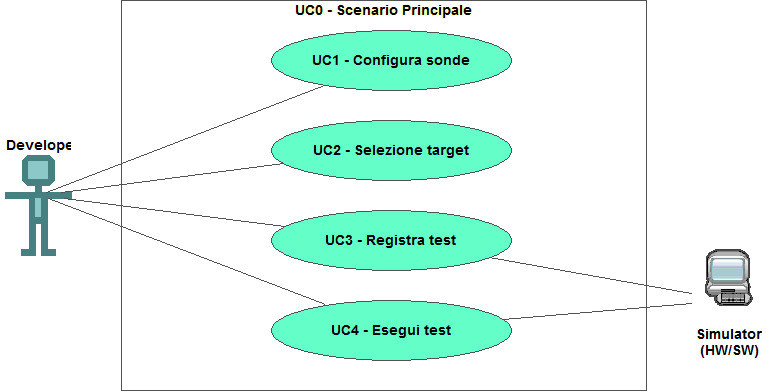
\includegraphics[alt={Testo alternativo dell'immagine}, width=0.75\columnwidth]{img/usecase/scenario-principale.jpeg}
    \caption{Use Case 0: Scenario principale}
    \label{fig:scenario_principale}
\end{figure}

\begin{usecase}{0}{Scenario principale}
    \usecaseactors{Sviluppatore applicativi.}
    \usecasepre{Lo sviluppatore è entrato nel plugin di simulazione all'interno dell'IDE.}
    \usecasedesc{La finestra di simulazione mette a disposizione i comandi per configurare, registrare o eseguire un test.}
    \usecasepost{Il sistema è pronto per permettere una nuova interazione.}
    \label{uc:uc_scenario_principale}
\end{usecase}

\begin{usecase}{1}{Gestione Utente}
    \usecaseactors{Amministratore, Utente Registrato.}
    \usecasepre{L'utente deve essere autenticato nel sistema.}
    \usecasedesc{L'utente può gestire le informazioni del proprio profilo.}
    \usecasepost{Le modifiche vengono salvate nel sistema.}
    \usecasealt{Se l'utente non è autenticato, visualizza un messaggio di errore.}
    \label{uc:uc_casi_uso}
\end{usecase}

\begin{usecase}{2}{Creazione Prodotto}
    \usecaseactors{Amministratore.}
    \usecasepre{L'amministratore ha effettuato l'accesso al sistema.}
    \usecasedesc{L'amministratore può aggiungere un nuovo prodotto al catalogo.}
    \usecasepost{Il nuovo prodotto viene aggiunto con successo.}
    \usecasealt{Se i campi obbligatori non sono compilati, visualizza un messaggio di errore.}
    \label{uc:uc_creazione_prodotto}
\end{usecase}

\section{Tracciamento dei requisiti}
Da un'attenta analisi dei requisiti e degli use case effettuata sul progetto è stata stilata la tabella che traccia i requisiti in rapporto agli use case.\\
Sono stati individuati diversi tipi di requisiti e si è quindi fatto utilizzo di un codice identificativo per distinguerli.\\
Il codice dei requisiti, dove ogni requisito è identificato con il carattere \textbf{R}, è così strutturato:
\begin{enumerate}
    \item[\textbf{F}:] Funzionale.
    \item[\textbf{Q}:] Qualitativo.
    \item[\textbf{V}:] Di vincolo.
    \item[\textbf{N}:] Obbligatorio (necessario).
    \item[\textbf{D}:] Desiderabile.
    \item[\textbf{Z}:] Opzionale.
\end{enumerate}

Nelle tabelle \ref{tab:requisiti_funzionali}, \ref{tab:requisiti_qualitativi} e \ref{tab:requisiti_vincolo} sono riassunti i requisiti e il loro tracciamento con gli use case delineati in fase di analisi.

\section{Tabelle dei requisiti}
\begin{center}
    \rowcolors{1}{}{tableGray}
    \begin{longtable}{|p{2.25cm}|p{7.75cm}|p{2.25cm}|}
    \hline
    %\rowcolor{hyperColor!5}
    \multicolumn{1}{|c|}{\textbf{Requisito}} & \multicolumn{1}{c|}{\textbf{Descrizione}} & \multicolumn{1}{c|}{\textbf{Use Case}}\\
    \hline 
    \endfirsthead
    \rowcolor{white}
    \multicolumn{3}{c}{{\bfseries \tablename\ \thetable{} -- Continuo della tabella}}\\
    \hline
    %\rowcolor{hyperColor!5}
    \multicolumn{1}{|c|}{\textbf{Requisito}} & \multicolumn{1}{c|}{\textbf{Descrizione}} & \multicolumn{1}{c|}{\textbf{Use Case}}\\
    \hline 
    \endhead
    \hline
    \rowcolor{white}
    \multicolumn{3}{|r|}{{Continua nella prossima pagina...}}\\
    \hline
    \endfoot
    \endlastfoot
    
    RFN-1 & L’interfaccia permette di configurare il tipo di sonde del test & UC1 \\
    \hline
    \hiderowcolors
    \caption{Tabella del tracciamento dei requisiti funzionali.}
    \label{tab:requisiti_funzionali}
    \end{longtable}
\end{center}

\begin{center}
    \rowcolors{1}{}{tableGray}
    \begin{longtable}{|p{2.25cm}|p{7.75cm}|p{2.25cm}|}
    \hline
    %\rowcolor{hyperColor!5}
    \multicolumn{1}{|c|}{\textbf{Requisito}} & \multicolumn{1}{c|}{\textbf{Descrizione}} & \multicolumn{1}{c|}{\textbf{Use Case}}\\
    \hline 
    \endfirsthead
    \rowcolor{white}
    \multicolumn{3}{c}{{\bfseries \tablename\ \thetable{} -- Continuo della tabella}}\\
    \hline
    %\rowcolor{hyperColor!5}
    \multicolumn{1}{|c|}{\textbf{Requisito}} & \multicolumn{1}{c|}{\textbf{Descrizione}} & \multicolumn{1}{c|}{\textbf{Use Case}}\\
    \hline 
    \endhead
    \hline
    \rowcolor{white}
    \multicolumn{3}{|r|}{{Continua nella prossima pagina...}}\\
    \hline
    %\caption{Tabella del tracciamento dei requisiti qualitativi.}
    \endfoot
    \endlastfoot
    
    RQD-1n & Le prestazioni del simulatore hardware deve garantire la giusta esecuzione dei test e non la generazione di falsi negativi & - \\
    \hline
    RQD-1n & Le prestazioni del simulatore hardware deve garantire la giusta esecuzione dei test e non la generazione di falsi negativi & - \\
    \hline
    RQD-1n & Le prestazioni del simulatore hardware deve garantire la giusta esecuzione dei test e non la generazione di falsi negativi & - \\
    \hline
    RQD-1n & Le prestazioni del simulatore hardware deve garantire la giusta esecuzione dei test e non la generazione di falsi negativi & - \\
    \hline
    RQD-1n & Le prestazioni del simulatore hardware deve garantire la giusta esecuzione dei test e non la generazione di falsi negativi & - \\
    \hline
    RQD-1n & Le prestazioni del simulatore hardware deve garantire la giusta esecuzione dei test e non la generazione di falsi negativi & - \\
    \hline
    \hiderowcolors
    \caption{Tabella del tracciamento dei requisiti qualitativi.}
    \label{tab:requisiti_qualitativi}
    \end{longtable}
\end{center}

\begin{center}
    \rowcolors{1}{}{tableGray}
    \begin{longtable}{|p{2.25cm}|p{7.75cm}|p{2.25cm}|}
    \hline
    %\rowcolor{hyperColor!5}
    \multicolumn{1}{|c|}{\textbf{Requisito}} & \multicolumn{1}{c|}{\textbf{Descrizione}} & \multicolumn{1}{c|}{\textbf{Use Case}}\\
    \hline 
    \endfirsthead
    \rowcolor{white}
    \multicolumn{3}{c}{{\bfseries \tablename\ \thetable{} -- Continuo della tabella}}\\
    \hline
    %\rowcolor{hyperColor!5}
    \multicolumn{1}{|c|}{\textbf{Requisito}} & \multicolumn{1}{c|}{\textbf{Descrizione}} & \multicolumn{1}{c|}{\textbf{Use Case}}\\
    \hline 
    \endhead
    \hline
    \rowcolor{white}
    \multicolumn{3}{|r|}{{Continua nella prossima pagina...}}\\
    \hline
    \endfoot
    \endlastfoot
    
    RVO-1 & La libreria per l'esecuzione dei test automatici deve essere riutilizzabile & - \\
    \hline
    \hiderowcolors
    \caption{Tabella del tracciamento dei requisiti di vincolo.}
    \label{tab:requisiti_vincolo}
    \end{longtable}
\end{center}

\newpage
    \chapter{Progettazione e codifica}
\label{chap:progettazione-codifica}
Breve introduzione al capitolo

\section{Tecnologie e strumenti}
\label{sec:tecnologie-strumenti}
Di seguito viene data una panoramica delle tecnologie e strumenti utilizzati.

\subsection*{Tecnologia 1}
Descrizione Tecnologia 1.

\subsection*{Tecnologia 2}
Descrizione Tecnologia 2

\section{Ciclo di vita del software}
\label{sec:ciclo-vita-software}

\section{Progettazione}
\label{sec:progettazione}

\subsection{Namespace 1}
Descrizione namespace 1.

\section{Design Pattern utilizzati}

\section{Codifica}
Blocco di codice in C
\begin{listing}[H]
\begin{minted}{c}
#include <stdio.h>
int main() {
    print("Hello, world!");
    return 0;
}
\end{minted}
\caption{Example of code}
\label{listing:c}
\end{listing}

\newpage
    \chapter{Processi e metodologie}
\label{chap:processi-metodologie}

Lorem ipsum dolor sit amet, consectetuer adipiscing elit. Aenean commodo ligula eget dolor. Aenean massa. Cum sociis natoque\footnote{\cite{site:agile-manifesto}} penatibus et magnis dis parturient montes, nascetur ridiculus mus. Donec quam felis, ultricies nec\footnote{\cite{article:spooky}}, pellentesque eu, pretium quis, sem.

\begin{figure}[H]
    \centering
    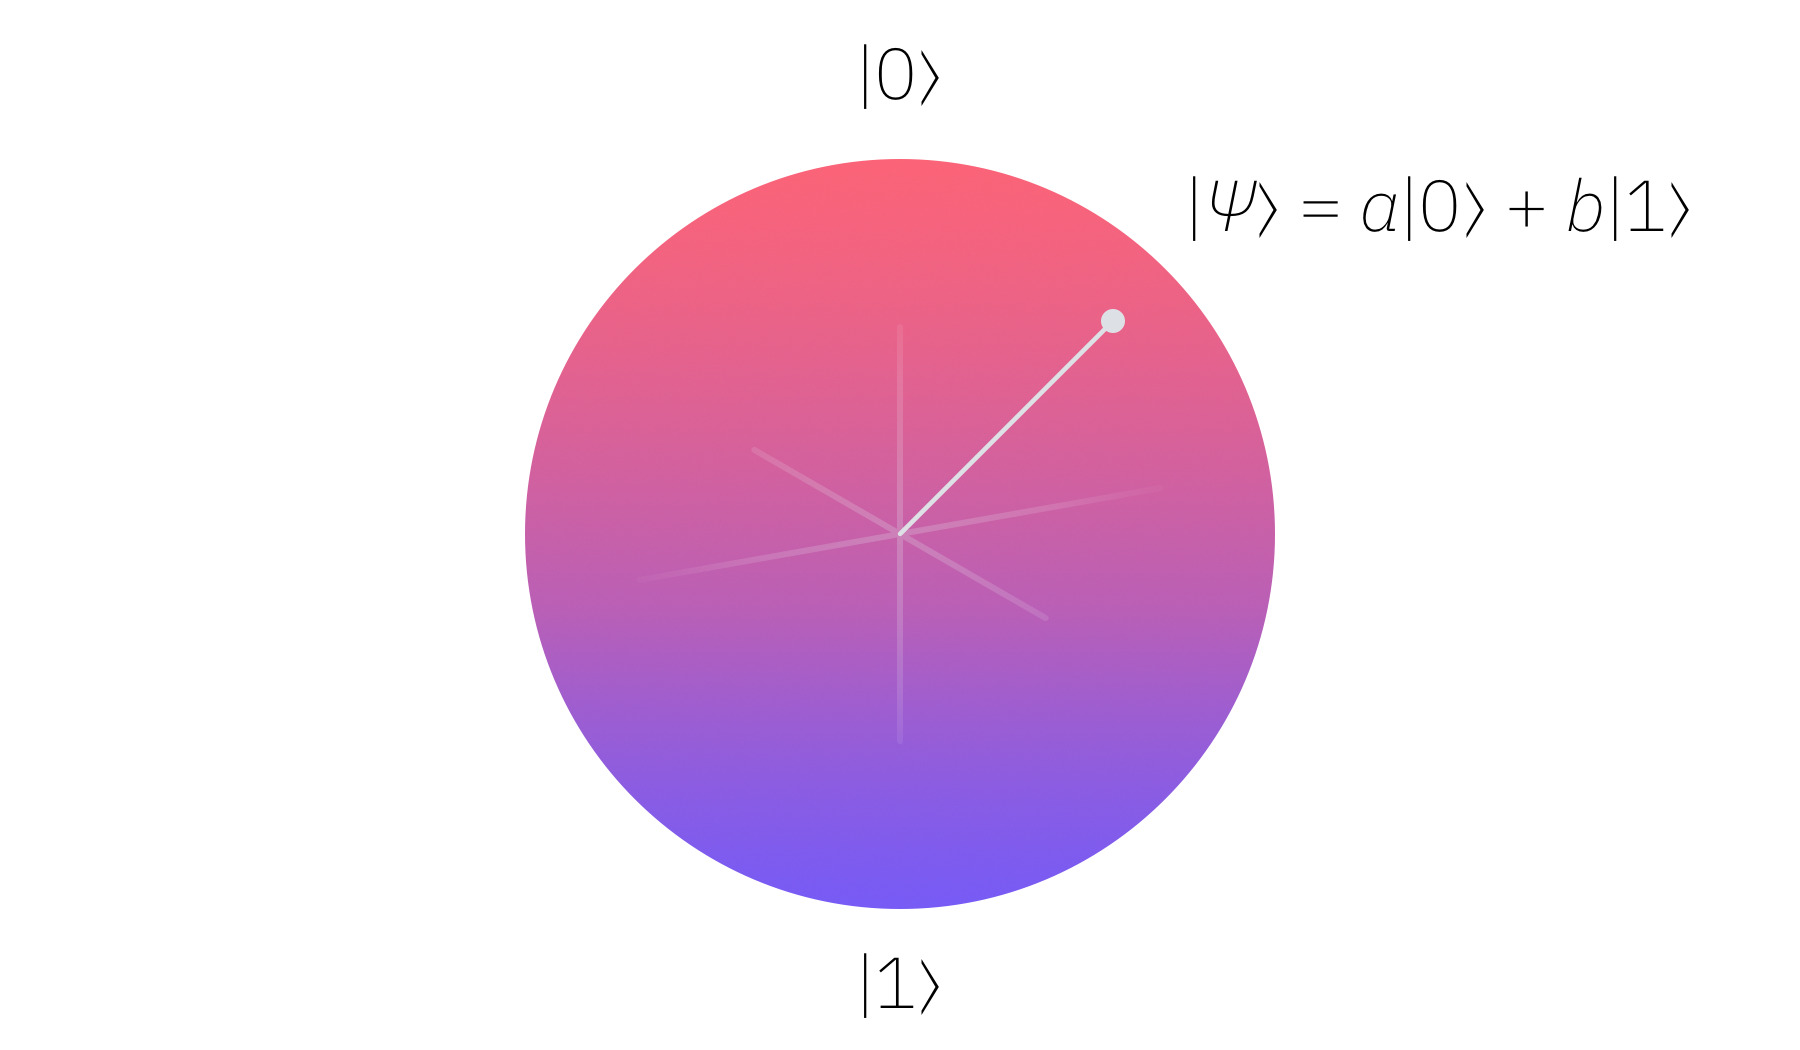
\includegraphics[alt={Testo alternativo dell'immagine}, height=5cm]{img/qubit.jpeg}
    \description[Rappresenzazione Qubit]{Long description}
    \caption{Lorem}
    \label{fig:qubit}
\end{figure}
\lipsum[1]

\section{Processo sviluppo prodotto}
\lipsum[1-2]

\begin{listing}[H]
\begin{minted}{c}
#include <stdio.h>
int main() {
    print("Hello, world!");
    return 0;
}
\end{minted}
\caption{Example of code}
\label{listing:b}
\end{listing}

Lorem ipsum:
\begin{listing}[H]
\begin{minted}{c}
#include <stdio.h>
int main() {
    print("Hello, world!");
    return 0;
}
\end{minted}
\caption{Example of code}
\label{listing:b-2}
\end{listing}

Lorem ipsum:
\begin{listing}[H]
\begin{minted}{c}
#include <stdio.h>
int main() {
    print("Hello, world!");
    return 0;
}
\end{minted}
\caption{Example of code}
\label{listing:b-3}
\end{listing}

\newpage
    \chapter{Verifica e validazione}
\label{chap:verifica-validazione}

\begin{figure}[H]
    \centering
    
\includegraphics[alt={Testo alternativo dell'immagine}, width=1\columnwidth]{img/quantum_superposition.jpeg}
    \caption{Lorem}
    \label{fig:enter-label}
\end{figure}

\lipsum[1-2]

Lorem ipsum:
\begin{listing}[H]
\begin{minted}{python}
def recur_fibo(n):
   if n <= 1:
       return n
   else:
       return(recur_fibo(n-1) + recur_fibo(n-2))
nterms = 10
if nterms <= 0:
   print("Plese enter a positive integer")
else:
   print("Fibonacci sequence:")
   for i in range(nterms):
       print(recur_fibo(i))
\end{minted}
\caption{Fibonacci recursive}
\label{listing:py_fibo}
\end{listing}

\lipsum[1]

\newpage
    \chapter{Conclusioni}
\label{chap:conclusioni}

\section{Consuntivo finale}
Ipsum

\section{Raggiungimento degli obiettivi}
Sit amet

\section{Conoscenze acquisite}

For applying a subscripting G:\\
Lorem \gls{sdkg}\glox ispum dolor.\\
If the G is followed by a punctuation, such as a "." like in this example, you need to use \textit{gloxspacing}\\
Lorem \gls{sdk}\glox\gloxspacing.\\
Otherwise...\\
Lorem \gls{sdkg}\glox.\\
The "." is not placed in the correct place.\\
Lorem Ipsum dolor \gls{sdkg}\glox\gloxspacing, sit amet.\\
Lorem \gls{apig}

\section{Valutazione personale}
Lorem \gls{umlg}\glox\gloxspacing, ipsum dolor sit amet

\section{Valutazione personale}
Lorem Ipsum dolor Lorem \gls{sdk}

\newpage

    \pagenumbering{roman}
    \backmatter
    \chapter{Bibliografia}
\label{cap:bibliography}

\nocite{*}

% % Books bibliography
% \printbibliography[heading=subbibliography, title={Testi}, type=book]

% % Articles bibliography
% \printbibliography[heading=subbibliography, title={Articoli}, type=article]

% Websites bibliography
\printbibliography[heading=subbibliography, title={Siti}, type=online]

    \chapter{Sitografia}
\label{cap:webliography}
\nocite{*}

% Websites bibliography
\printbibliography[heading=subbibliography, title={\null}, type=online]

\end{document}